\chapter{The Estimators and Simulator}

\chapauthor{Stephen P. Hughes}{NASA/Goddard Space Flight Center}
\chapauthor{Darrel J. Conway}{Thinking Systems, Inc.}
\chapauthor{Matthew P. Wilkins}{Schafer Corporation}

GMAT's Estimator classes are shown in Figure~\ref{fig:EstimatorClasses}.  The first estimator build of GMAT includes the blocks shaded orange in the diagram: the Estimator base class, the BatchEstimator intermediate class, and the BatchLeastSquares estimator.  The second build adds the Filter intermediate class and a Kalman filter based estimator to the system.  Potential extensions to this class hierarchy are shown in the figure as well.

\begin{figure}[htbp]
\begin{center}
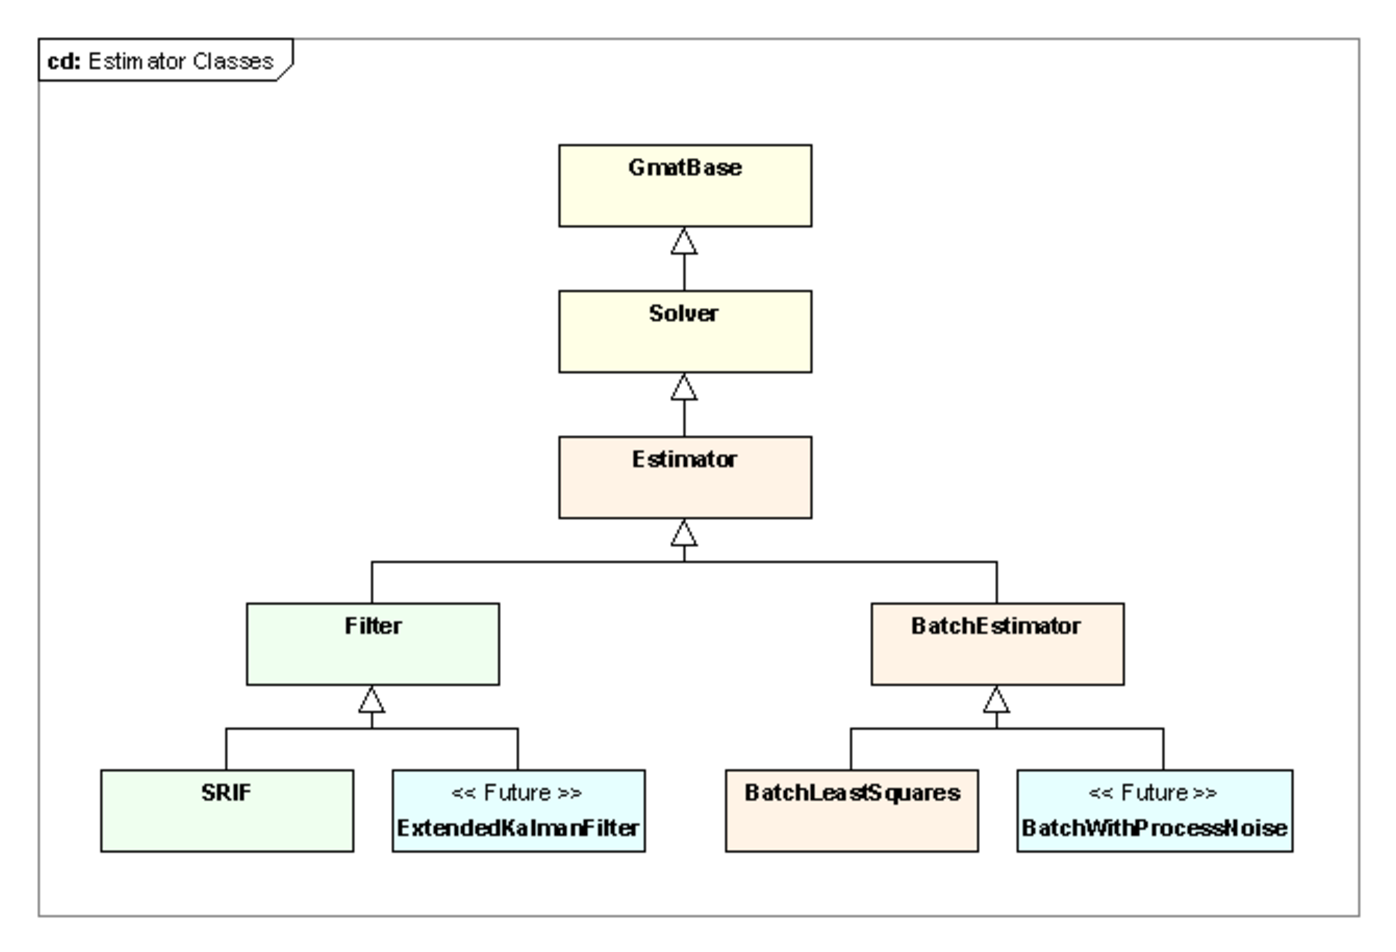
\includegraphics[scale=0.6]{Images/EstimatorClasses.eps}
\caption{\label{fig:EstimatorClasses}Classes in GMAT's Estimator Hierarchy}
\end{center}
\end{figure}

GMAT's Estimator base class defines the core functionality shared by all estimators.  It includes the top level Estimator interfaces, initialization code for the shared elements including the EstimationStateManager and MeasurementManager, and the member components implementing these elements.  The interfaces in this class are defined so that the estimation commands can treat the estimator process generically, and therefore drive the estimation process without intimate knowledge of the algorithm that is implemented in the estimator.

GMAT's estimator classes are derived from the Solver base class.  The Solver class provides data structures and methods designed so that derived classes can implement a finite state\footnote{``State'' in the context of a finite state machine corresponds to the status of the machine.  This is distinct from the state vector used by an estimator or SpaceObject.  When the context does not make the distinction clear, the term ``finite state'' is used for the state machine states and ``state vector'' for the data.} machine that, together with a matching command, organizes the process of working with the elements of the a GMAT mission to drive the algorithm implemented in the solver.  The command portion of this partnership manages the interface with the Sandbox and the propagation subsystem, and, when appropriate, with a solver control sequence designed to provide a sequence of commands when that sequence involves more than just direct propagation.  The solver side of the partnership manages the state of the solution algorithm.  That state is represented by one of several distinct values; hence the state machine is called a finite state machine.  The command side retrieves the state if the state machine from the solver, performs any necessary control sequence actions, and then passes control to the solver so that the solver can evaluate and potentially change state based on the results of the command's actions.

The state machine in GMAT's solvers provides a mechanism to ensure that the control sequence is executed in a sensible manner for the implemented algorithm.  As such, each derived solver class will define its state machine to meet the needs of its algorithm.  The state machines for each of the new estimators are described in the corresponding class descriptions below.

The following sections describe each estimation class in the figure, starting with the Estimator base class.  The capabilities and member elements are described, along with the processes that each class implements.

\section{The Estimator Base Class}

The Estimator class contains two key member objects used by all of GMAT's estimators: an instance of the EstimationStateManager and an instance of the MeasurementManager.  The details of those classes are provided in the corresponding sections of this document.  In this section you will see how these objects are set up and used by the Estimator classes.

Figure~\ref{fig:EstimatorClassDetails} shows the Estimator class, its ancestors, and its predecessor. The details of the class contents are shown in this figure, along with the helper classes mentioned above.  The Estimator class centralizes the interfaces to the measurement data and the estimation state vector, along with the other elements that all estimators need.  This class extends the features of the Solver class by adding and initializing these new elements.  As a base class, we anticipate that the implementation process for the derived estimators will result in a fair amount of refactoring, particularly as the BatchEstimator and Filter classes are implemented, consolidating additional common estimation features.

\begin{figure}[htbp]
\begin{center}
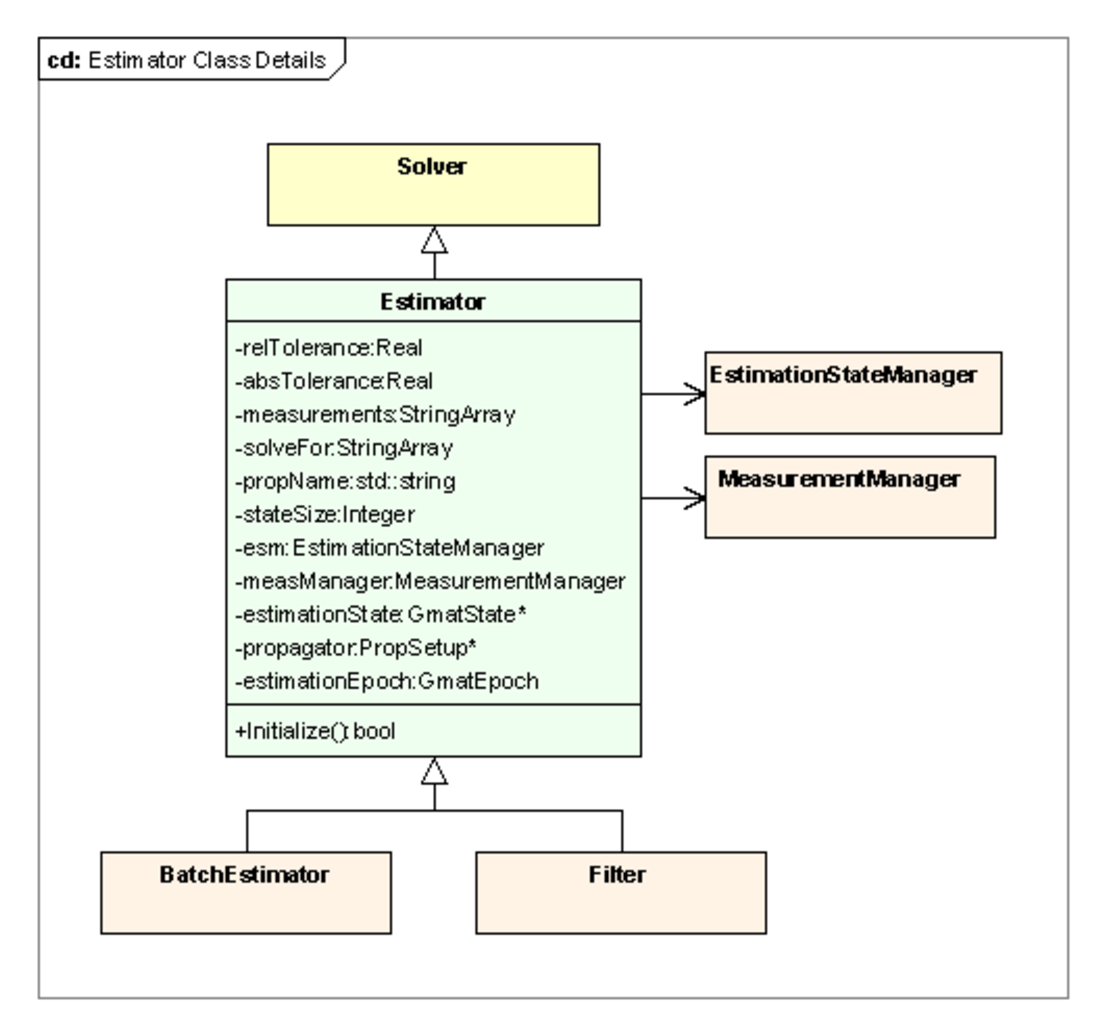
\includegraphics[scale=0.6]{Images/EstimatorClassDetails.eps}
\caption{\label{fig:EstimatorClassDetails}The Estimator Class}
\end{center}
\end{figure}

\subsection{Key Processes}

The Estimator base class has one key process: the Initialize method, which  initializes its management members and prepares its propagation subsystem for initialization.

\subsubsection{Estimator Initialization}

The Estimator class manages the initialization of the EstimationStateManager and the MeasurementManager, along with preparation of the PropagationStateManager for initialization, as is shown in Figure~\ref{fig:EstimatorInitialize}.  The Estimator::Initialize() method calls the Solver::Initialize() method first to ensure that the Solver data structures are properly prepared for use.  Following this call, the EstimationStateManager::Initialize() method is called, which sets the data structures for the estimation state vector and then builds the vector.  Once the estimation state vector has been built, the Estimator walks through the estimation state vector and passes each element that needs propagation into the PropagationStateManager assigned to the Estimator's propagator.  This process prepares the propagation subsystem for initialization, but does not perform the actual initialization.  That call is made in the estimation command immediately prior to execution so that all transient forces required for the propagation can be managed.  Finally, the MeasurementManager::Initialize() method is called, causing the measurement manager to read all of the data available for processing and to build the structures needed for that processing.  This step completes initialization for the Estimator base class.

\begin{figure}[htbp]
\begin{center}
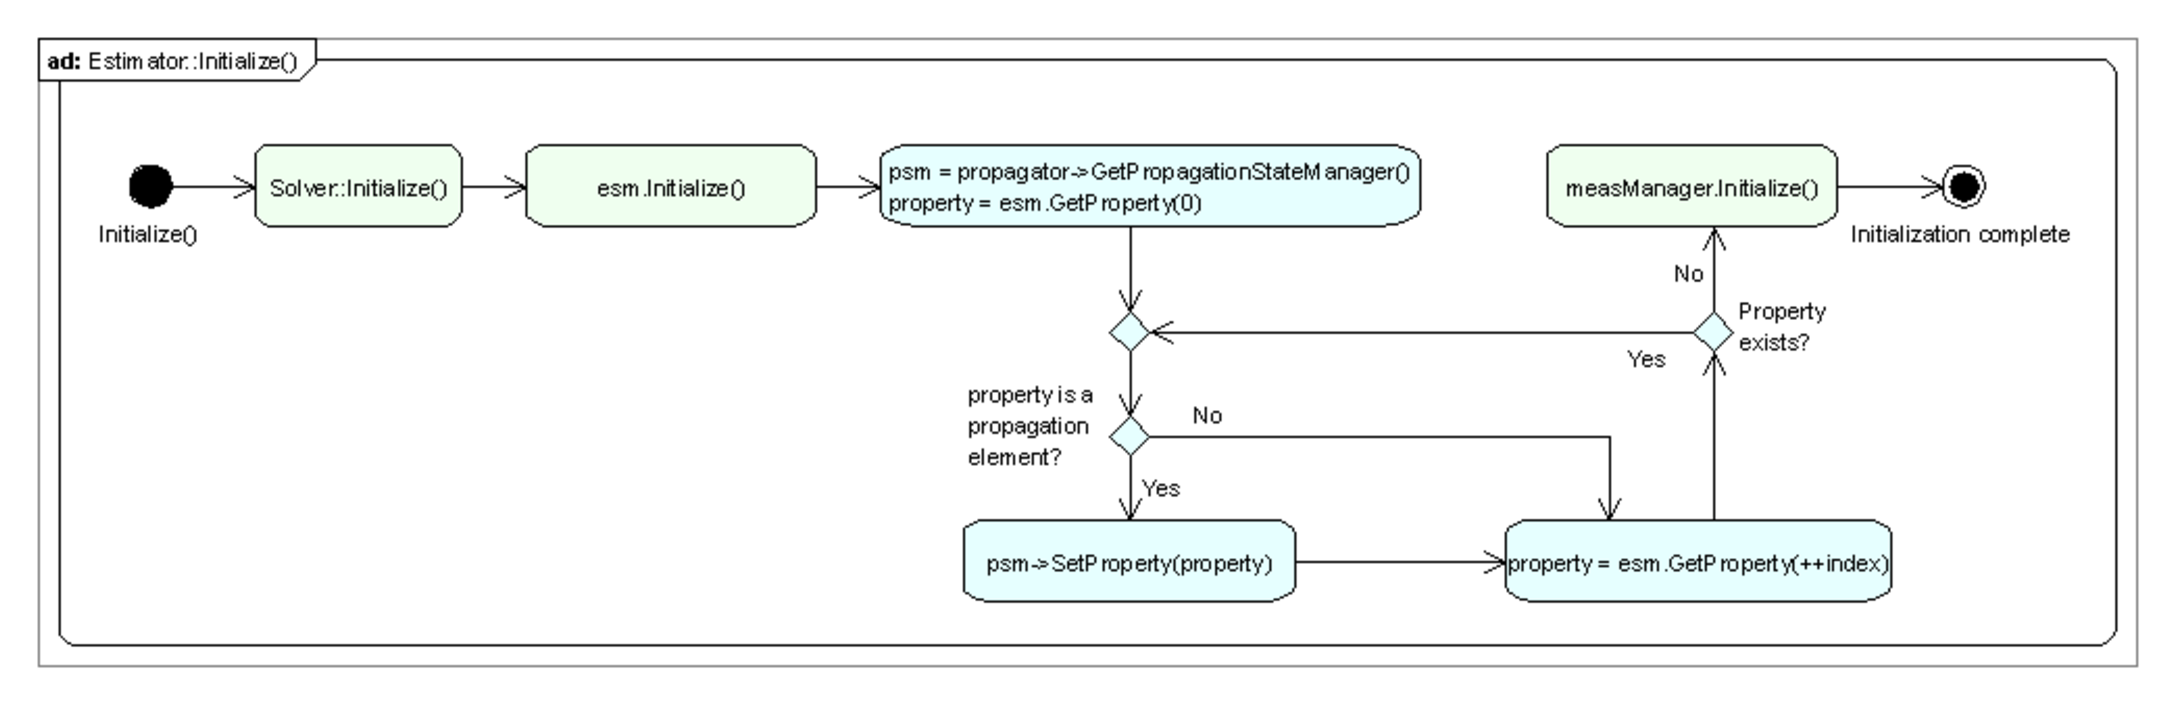
\includegraphics[scale=0.45]{Images/EstimatorInitialize.eps}
\caption{\label{fig:EstimatorInitialize}Estimator Class Initialization}
\end{center}
\end{figure}

\subsection{Estimator Members}

\paragraph{Estimator Attributes}

\begin{itemize}
\item \textbf{Real relTolerance}:  The maximum change from the previous RMS error in the residuals to the current RMS error allowed in order for convergence to be met.
\item \textbf{Real absTolerance}:  The largest allowed change in the estimation state in order for convergence to be met.
\item \textbf{StringArray measurements}:  Names of the measurement types used in this estimator.  This array of names is passed to the MeasurementManager for processing.
\item \textbf{StringArray solveFor}:  List of the solve for parameters used in the estimator.
\item \textbf{std::string propName}:  Name of the configured propagator used to evolve objects during the estimation process.
\item \textbf{Integer stateSize}:  The size of the estimation state vector.
\item \textbf{EstimationStateManager esm}:  The EstimationStateManager for the estimator.  This member is responsible for the communications between GMAT's objects and the data structures manipulated by the estimator during the estimation process.
\item \textbf{MeasurementManager measManager}:  The MeasurementManager for the estimator.  This object is responsible for managing all of the measurement objects in the estimation process.  It is an intermediary responsible for retrieving observed and calculated data, and supplying those data to the estimator.
\item \textbf{GmatState *estimationState}:  A pointer to the estimation state managed by the EstimationStateManager.  This pointer is set after the EstimationStateManager is initialized.  It is provided for convenience, so that repeated calls to esm.GetState() are not needed in the code.
\item \textbf{PropSetup *propagator}:  The propagator configured for the estimation.
\item \textbf{GmatEpoch estimationEpoch}:  The estimation epoch.  For batch estimators, this epoch is the epoch of the state estimate.  For sequential epochs, it tracks the epoch of the current estimate.
\end{itemize}

\paragraph{Estimator Methods}

\begin{itemize}
\item \textbf{bool Initialize()}:  Prepares the EstimationStateManager and MeasurementManager for use in estimation, and loads the propagator's PropagationStateManager so it can be initialized by the propagation enabled commands.
\end{itemize}

\section{The BatchEstimator Class}

\begin{figure}[htbp]
\begin{center}
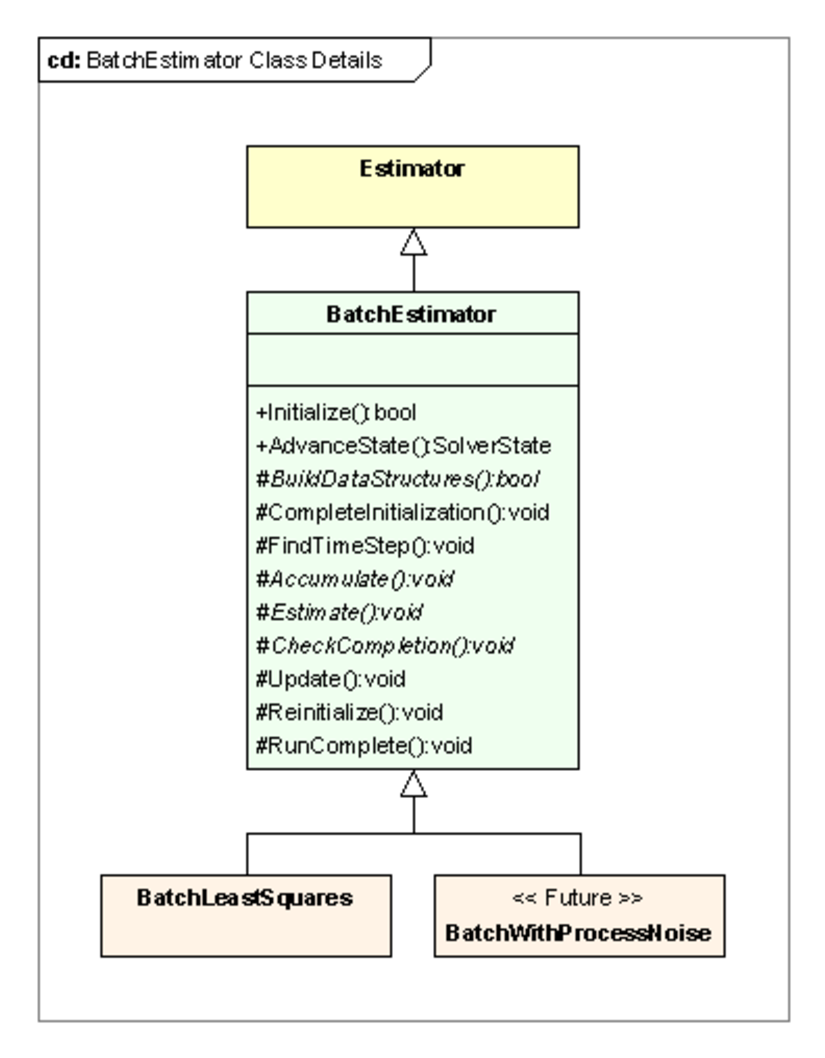
\includegraphics[scale=0.6]{Images/BatchEstimatorClassDetails.eps}
\caption{\label{fig:BatchEstimatorClassDetails}The BatchEstimator Class}
\end{center}
\end{figure}

The BatchEstimator class, shown in Figure~\ref{fig:BatchEstimatorClassDetails}, implements the infrastructure used by GMAT's batch estimators.  This infrastructure includes the implementation of a state machine intended to support the usual sequence of actions needed for batch estimation. The class defines with the methods called from this state machine, and provides implementations of the methods that are considered to be common to the batch estimation process.  All of the common methods implemented for the BatchEstimator class are declared virtual.  Derived classes can override the estimation state machine or any of the implemented methods as needed to support algorithm specific needs.  The Accumulate(), Estimate(), and CheckCompletion() methods are considered to always be implementation specific, and therefore must be implemented in the classes derived from the BatchEstimator class.

\subsection{Key Processes}

The BatchEstimator class implements a basic finite state machine that follows a typical batch estimation process.  There are two processes that work together to implement the state machine: initialization of the BatchEstimator and execution of the finite state machine.

\subsubsection{Initialization}

The initialization process in the Sandbox starts with the object setting phase described in the GMAT run overview.  At the end of this phase, all of the references objects have been set on the BatchEstimator object, and it is ready to validate those objects and set the pointers for use in the estimation process.  This process is shown in Figure~\ref{fig:BatchEstimatorInitialize}.

\begin{figure}[htbp]
\begin{center}
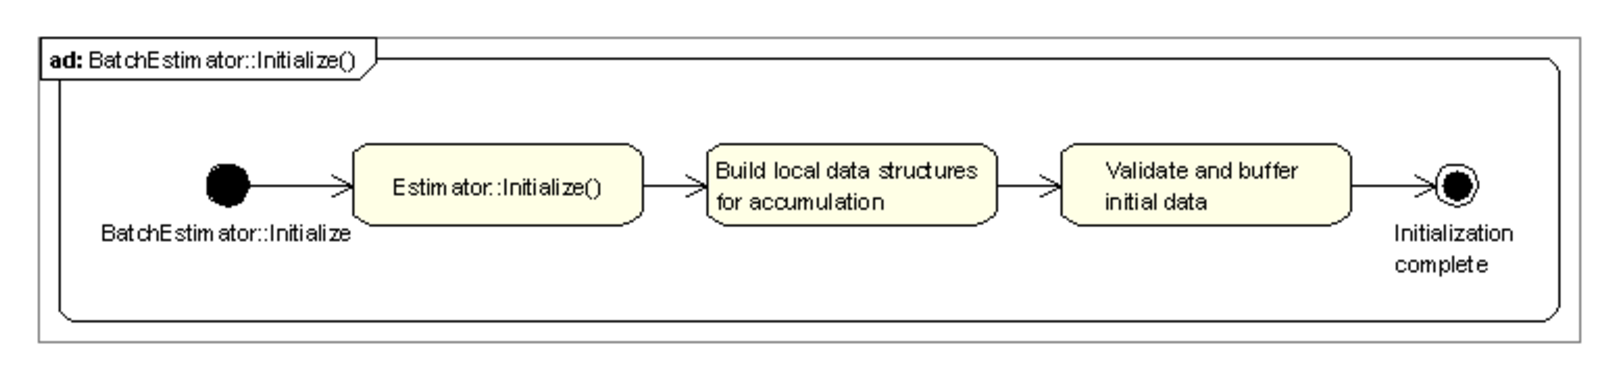
\includegraphics[scale=0.6]{Images/BatchEstimatorInitialize.eps}
\caption{\label{fig:BatchEstimatorInitialize}Initialization in the BatchEstimator Class}
\end{center}
\end{figure}

The initialization process for the BatchEstimator starts by initializing the Estimator base class as described above.  Once that process completes successfully, the data structures required for accumulation are prepared.  Finally, the initial data are checked to be sure that they contain all of the required data, and that these data are internally consistent, and they are buffered so they can be restored during iteration.  This completes the initialization process for the batch estimator.

\subsubsection{Estimation State Machine}

Figure~\ref{fig:BatchEstimatorOverview} shows the estimation process implemented in the BatchEstimator class.  The batch estimator state machine is shown in the lower partition in the figure, while the actions performed by the command running the state machine are shown in the upper partition.  The state machine implementation is key to the estimation process in GMAT, so it will be described in some detail in the following paragraphs.

\begin{figure}[htbp]
\begin{center}
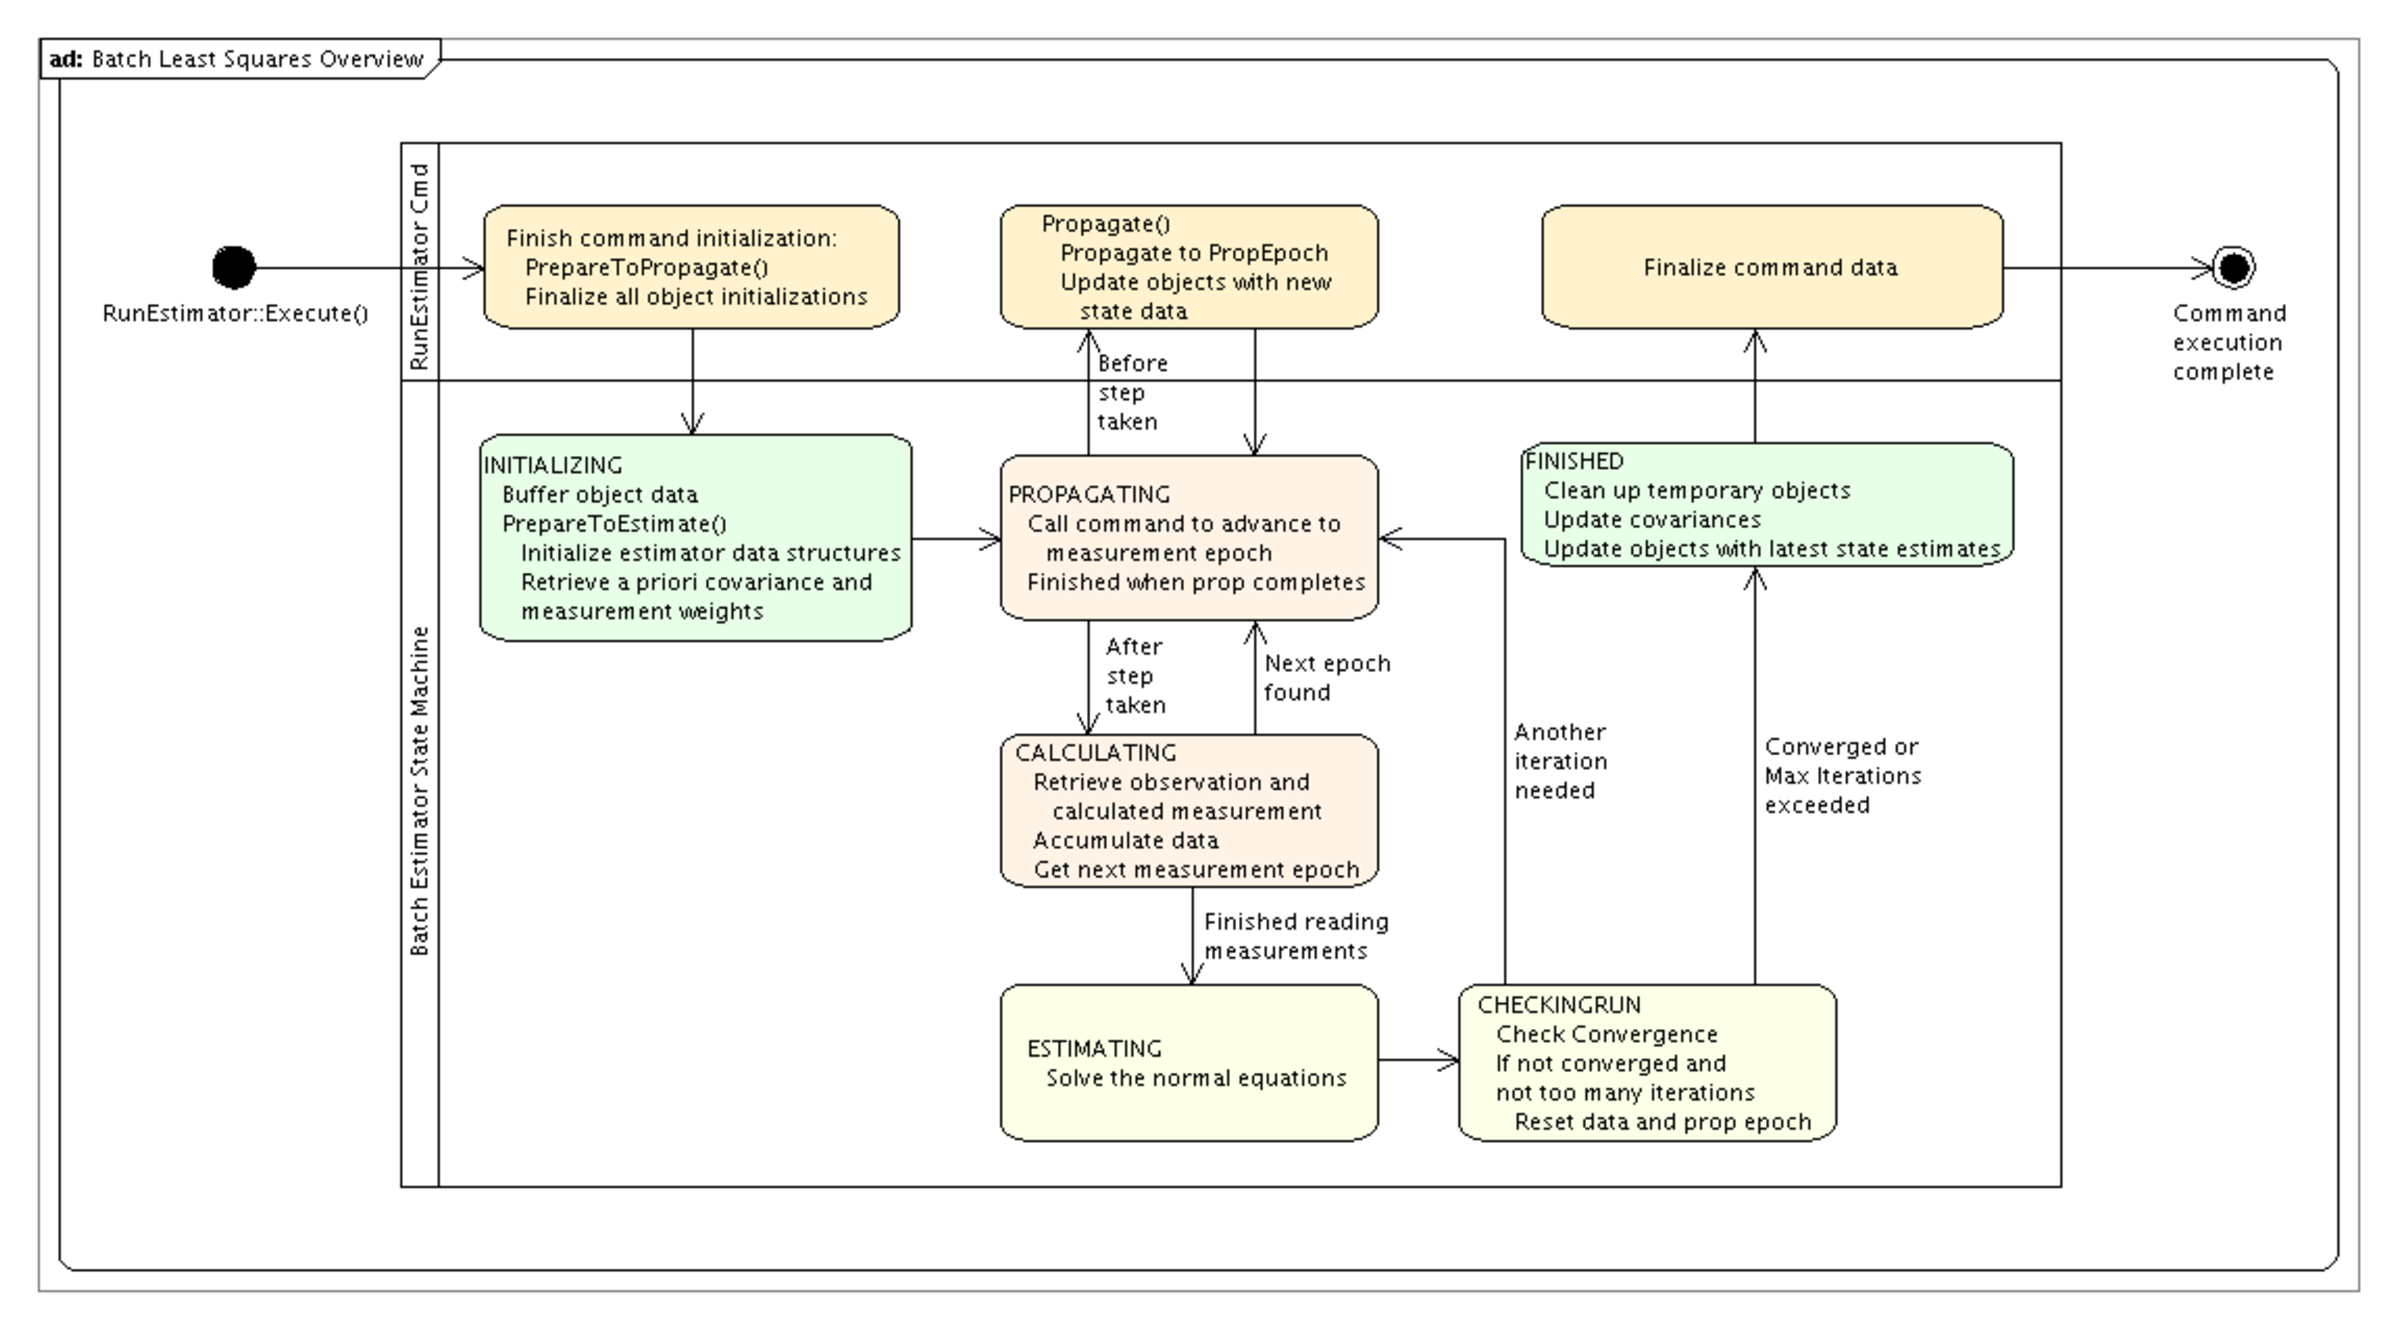
\includegraphics[scale=0.4]{Images/BatchLeastSquaresOverview.eps}
\caption{\label{fig:BatchEstimatorOverview}Performing Batch Estimation}
\end{center}
\end{figure}

\paragraph{GMAT's Solver State Machines}

GMAT's solver finite state machines are used to move the solution algorithm through the steps required to apply the algorithm to the objects that are used to solve a user specified problem. Each step of the process is represented by a discrete numerical identifier, referred to as the state of the process.  That identifier is used to specify a set of actions that, when performed, prepare the finite state machine to advance from its current state to the next state in the solution process.  The state identifiers are defined in a C++ enumeration, the SolverState enumeration in the Gmat namespace.

Each state in the solver state machine performs actions designed to move the elements of GMAT from their entry condition to the condition required to advance to the next state.  GMAT advances from one state to the next using the AdvanceState() method on the solver.  When AdvanceState() is called, the solver executes a method assigned to the state and reports the results to the solver's text file.  The method call is responsible for running the actions assigned to the state, and then determining the next state and changing the state identifier accordingly based on the results of the actions executed.

\paragraph{The BatchEstimator Finite State Machine}

The BatchEstimator uses seven states to drive its algorithm.  These seven states, shown in the bottom partition of Figure~\ref{fig:BatchEstimatorOverview}, work together to estimation a user defined state vector.  The list below describes each state of the machine, including the entry and exit conditions along with the internal actions required to move to the exit condition for the state:

\begin{description}
\item[INITIALIZING]\hspace{1pt}
\begin{itemize}
\item \textbf{Entry condition} The INITIALIZING state is the state the BatchEstimator takes upon completion of initialization in the Sandbox.  Upon completion of an estimation run, the BatchEstimator returns to this state so that a subsequent call can reuse the same estimator.
\item \textbf{Actions} \textit{Method Name: CompleteInitialization()}
\begin{itemize}
\item Determine if any observations are available; if not, abort estimation 
\item If necessary, propagate to estimation epoch
\item Gather the data and fill the batch estimator's state
\item Initialize the state transition matrix
\item Gather a priori covariances and measurement weights
\item Buffer all estimation objects
\end{itemize}
\item \textbf{Exit condition}
\begin{itemize}
\item Change to PROPAGATING state if an observation exists.  
\item Change to FINISHED state and post a warning message if none were found\footnote{The state machine in the figure shows the nominal path through the process.  Anomalous paths, like the absence of observation data mentioned here, are not included in the figure}.
\end{itemize}
\end{itemize}
\item[PROPAGATING]\hspace{1pt}
\begin{itemize}
\item \textbf{Entry condition}  An observation was found
\item \textbf{Actions} \textit{Method Name:  GetStepEpoch()}
\begin{itemize}
\item Determine time step for propagation to the observation epoch
\item Feed time step to command for propagation
\item Determine if measurement for the observation has events that require propagation
\end{itemize}
\item \textbf{Exit condition 1}
\begin{itemize}
\item Time step = 0
\item No unprocessed propagation events
\item Change state to CALCULATING
\end{itemize}
\item \textbf{Exit condition 2}
\begin{itemize}
\item Time step = 0
\item Events that require propagation not yet processed
\item Change state to LOCATING
\end{itemize}
\end{itemize}
\item[LOCATING]\hspace{1pt}
\begin{itemize}
\item \textbf{Entry conditions}
\begin{itemize}
\item An event that requires propagation has been found
\item Resources are at a known epoch for the event
\end{itemize}
\item \textbf{Actions} \textit{Method Name:  ProcessEvent(bufferData)}
\begin{itemize}
\item If bufferData is true, buffer state information
\item Calculate time step required for the event
\item Provide time step to command for propagation
\item Evaluate event to determine if propagation results are within tolerance
\item Iterate from time step calculation until event converges
\end{itemize}
\item \textbf{Exit condition 1}
\begin{itemize}
\item Event has converged
\item No additional events found
\item Reset state information to buffered data
\item Set bufferData flag to true
\item Change state to PROPAGATING
\end{itemize}
\item \textbf{Exit condition 2}
\begin{itemize}
\item Event has converged
\item Another event found
\item Set bufferData flag to false
\item Change state to LOCATING
\end{itemize}
\end{itemize}
\item[CALCULATING]\hspace{1pt}
\begin{itemize}
\item \textbf{Entry condition} Propagation and any required event location has been performed
\item \textbf{Actions} \textit{Method Name:  Accumulate()}
\begin{itemize}
\item Retrieve observation and calculated data
\item Accumulate the data
\item Retrieve the epoch of the next observation
\end{itemize}
\item \textbf{Exit condition 1}
\begin{itemize}
\item Another observation was found
\item Change state to PROPAGATING
\end{itemize}
\item \textbf{Exit condition 2}
\begin{itemize}
\item Final observation was processed
\item Change state to ESTIMATING
\end{itemize}
\end{itemize}
\item[ESTIMATING]\hspace{1pt}
\begin{itemize}
\item \textbf{Entry condition} All measurement data has been processed
\item \textbf{Actions} \textit{Method Name:  Estimate()}
\begin{itemize}
\item Solve the normal equations
\end{itemize}
\item \textbf{Exit condition}
\begin{itemize}
\item Estimation update generated
\item Change state to CHECKINGRUN
\end{itemize}
\end{itemize}
\item[CHECKINGRUN]\hspace{1pt}
\begin{itemize}
\item \textbf{Entry condition} An estimation update was generated
\item \textbf{Actions} \textit{Method Name:  CheckCompletion()}
\begin{itemize}
\item Check for convergence
\end{itemize}
\item \textbf{Exit condition 1}
\begin{itemize}
\item Estimation converged within tolerances
\item Change state to FINISHED
\end{itemize}
\item \textbf{Exit condition 2}
\begin{itemize}
\item Estimation did not converge
\item Maximum number of iterations exceeded
\item Change state to FINISHED
\end{itemize}
\item \textbf{Exit condition 3}
\begin{itemize}
\item Estimation did not converge
\item Maximum number of iterations not exceeded
\item Reset data and prop epoch through call to Reinitialize()
\item Update state with new estimate through call to Update()
\item Reset measurement iterator to point to first measurement
\item Change state to PROPAGATING
\end{itemize}
\end{itemize}
\item[FINISHED]\hspace{1pt}
\begin{itemize}
\item \textbf{Entry condition}  Estimation work finished
\item \textbf{Actions} \textit{Method Name:  RunComplete()}
\begin{itemize}
\item Update covariances
\item Update objects
\item Clean up data structures
\item Report convergence status
\end{itemize}
\item \textbf{Exit condition}
\begin{itemize}
\item Change state to INITIALIZING so estimator is reentrant
\end{itemize}
\end{itemize}
\end{description}

\subsection{BatchEstimator Members}

\paragraph{BatchEstimator Attributes}

The batch estimator does not have any additional attributes visible to the rest of the system.  The structures required for accumulation consist of vectors of the processed data required to solve the normal equations.  These data structures are algorithm specific, and are defined in the classes derived from the BatchEstimator class.

\paragraph{BatchEstimator Methods}

\begin{itemize}
\item \textbf{virtual bool Initialize()}:  Prepares the estimator for estimation.  The initialize method ensures that all of the top level components needed are present for the estimation process, and performs as much pre-run initialization as possible.
\item \textbf{virtual Gmat::SolverState AdvanceState()}:  Executions the  state machine actions necessary to move into a new state, and then advances the state to the next value in the finite state machine's process.
\item \textbf{virtual void CompleteInitialization()}:  Completes the initialization process, performs any necessary final propagation to move to the estimation epoch, and buffers the data that needs to be reset each time the batch process starts a new iteration.
\item \textbf{virtual void FindTimestep()}:  Compares the current state epoch with the next measurement epoch, and computes the time step -- in seconds -- that the propagator must apply to move from the current epoch to the measurement epoch.
\item \textbf{virtual void Update()}:  Applies corrections to the state to incorporate the changes necessary to build a new estimated state.
\item \textbf{virtual void Reinitialize()}:  Resets all of the buffered data so that a new iteration can be performed.
\item \textbf{virtual void RunComplete()}:  Finalizes all of the data, cleans up memory, and reports the estimation data.
\end{itemize}

\paragraph{BatchEstimator Abstract Methods}

The classes derived from the BatchEstimator class implement batch estimators that differ in the details of the estimator mathematics.  At a minimum, the derived classes must implement three methods: an Accumulate() method designed to collect the information needed from a pass through the measurement data, and Estimate() method that applies the batch algorithm to calculate state vector updates for the estimation state, and a CheckCompletion() method that tests the state updates and other criteria to determine if the estimation process should terminate.  These methods are listed here:

\begin{itemize}
\item \textbf{virtual bool BuildDataStructures() = 0}:  Method called by Initialize() to set up object specific data structures for the classes derived from the BatchEstimator class.
\item \textbf{virtual void Accumulate() = 0}:  Performs data accumulation for the batch algorithm.
\item \textbf{virtual void Estimate() = 0}:  Applies the batch algorithm to generate a new set of corrections to the estimation state vector at the estimation epoch.
\item \textbf{virtual void CheckCompletion() = 0}:  Checks to see if the estimation process should terminate, either because of convergence or for another reason.
\end{itemize}

\section{The BatchLeastSquares Class}

\begin{figure}[htbp]
\begin{center}
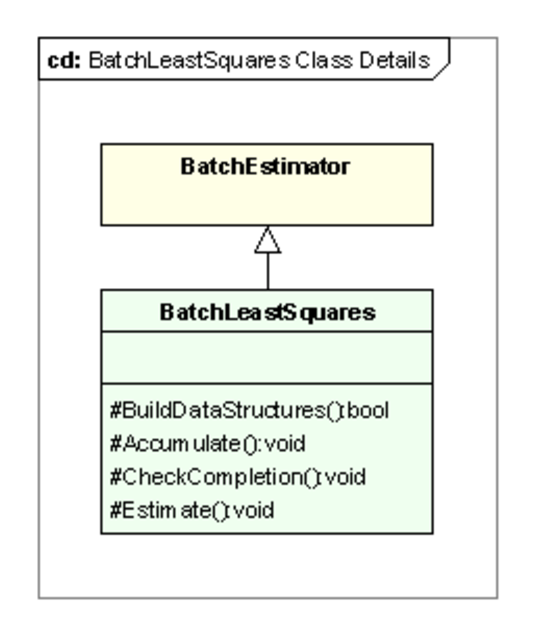
\includegraphics[scale=0.6]{Images/BatchLeastSquaresClassDetails.eps}
\caption{\label{fig:BatchLeastSquaresClass}The BatchLeastSquares Class}
\end{center}
\end{figure}

The BatchLeastSquares class, shown in Figure~\ref{fig:BatchLeastSquaresClass}, captures the mathematics of the accumulation and estimation processes.

\subsection{Key Processes}

The key processes performed by the BatchLeastSquares class are described in the parent class's text.  The BatchLeastSquares class does not provide any additional process level elements.  It does provide a specific implementation of the batch least squares algorithm, captured in the implementation of the four  abstract methods BuildDataStructures(), Accumulate(), Estimate(), and CheckCompletion().

\subsection{BatchLeastSquares Members}

\paragraph{BatchLeastSquares Attributes}

The BatchLeastSquares estimator does not require any new data members that need description at this level of the design.

\paragraph{BatchLeastSquares Methods}

\begin{itemize}
\item \textbf{virtual bool BuildDataStructures()}:  Method called by Initialize() to set up the data structures used for accumulation in the BatchLeastSquares estimator.
\item \textbf{virtual void Accumulate()}:  Collects the observed less calculated data and derivative information needed to build the normal equations.
\item \textbf{virtual void Estimate()}:  Solves the normal equations, generating the corrections that apply to the estimation state vector to construct a new estimate.
\item \textbf{virtual void CheckCompletion()}:  Checks the estimate to see if the estimation has converged or if another stopping criterion has been met.  If not, the most recent state corrections are applied to the estimation state vector.
\end{itemize}

\section{The Simulator Class}

GMAT's Simulator class is derived directly from the Solver class, and capitalizes on the state machine infrastructure provided by that class.  Simulators inherit these structures and use them to drive the simulation process. Figure~\ref{fig:SimulatorClass} shows the structure of the Simulator class, described in this section.

\begin{figure}[htbp]
\begin{center}
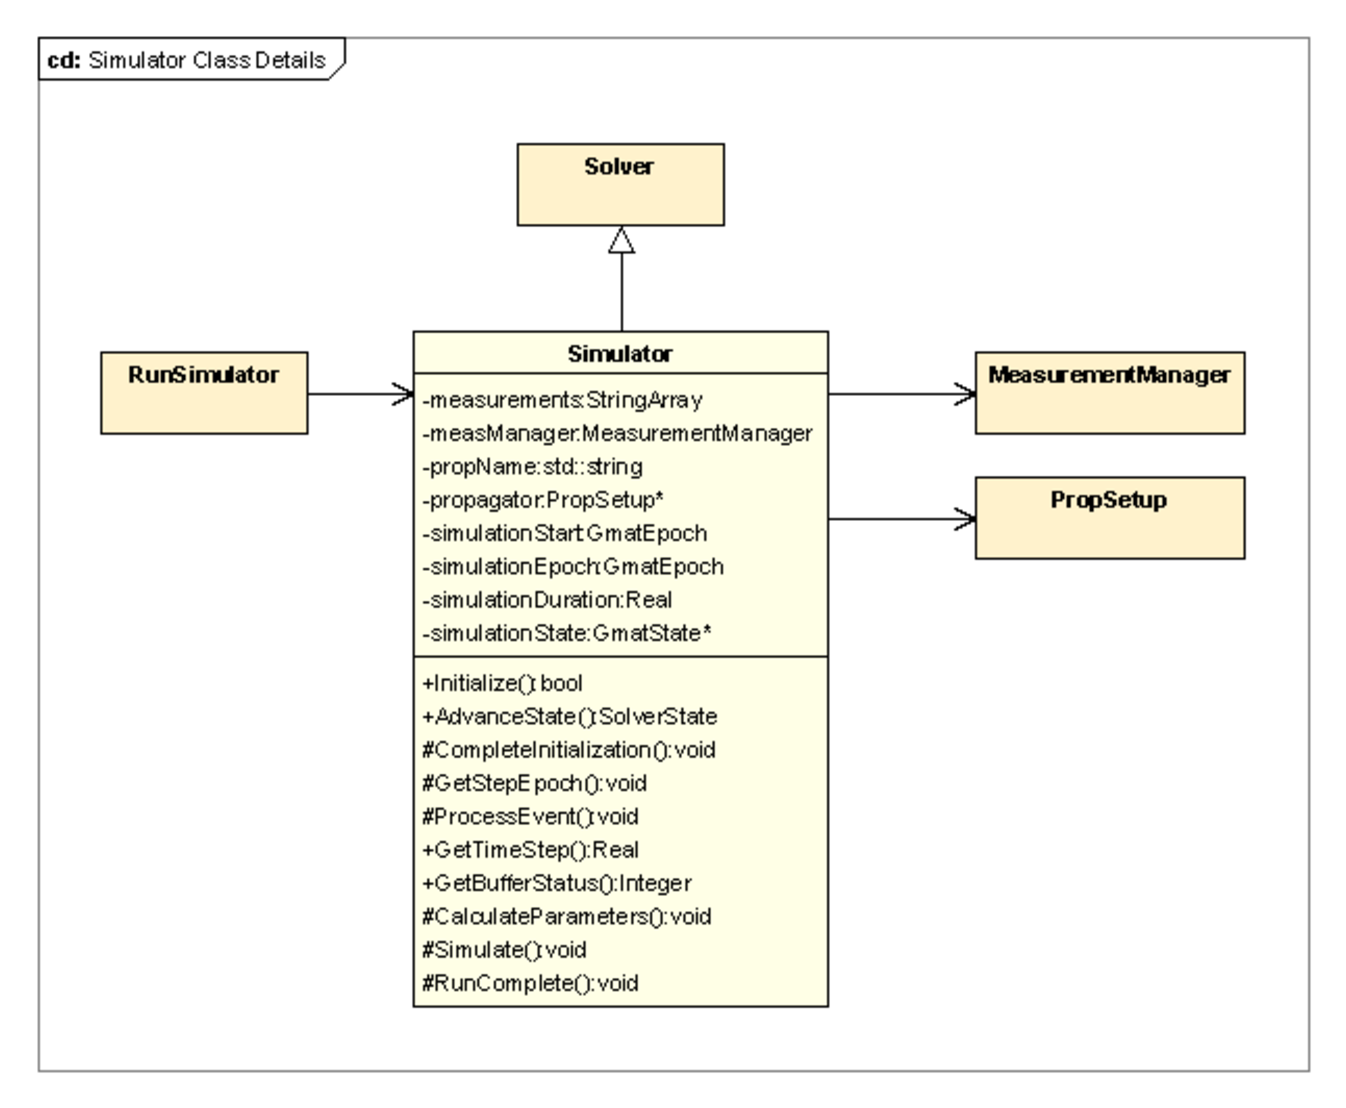
\includegraphics[scale=0.6]{Images/SimulatorClassDetails.eps}
\caption{\label{fig:SimulatorClass}The Simulator Class}
\end{center}
\end{figure}

\subsection{Key Processes}

The Simulator class has two key processes: the Initialize() method, which  initializes its management members and prepares its propagation subsystem for initialization, and the AdvanceState() method, which drives the simulation state machine.

\subsubsection{Simulator Initialization}

The initialization process manages the initialization of the MeasurementManager, PropSetup, and the referenced objects associated with these members.  The MeasurementManager initialization, described in the MeasurementManager class description, prepares the Measurement objects for use in the simulation.  The initialization for the PropSetup performs the pre-initialization steps so that the ODEModel and associated state data can be initialized at the start of the RunSimulator::Execute() call during the Mission Control Sequence run.

\subsubsection{The Simulation State Machine}

The Simulator uses six states to drive its algorithm.  These six states, shown in the bottom partition of Figure~\ref{fig:SimulatorStateMachine}, work together to simulate measurement data for a mission.

\begin{figure}[htbp]
\begin{center}
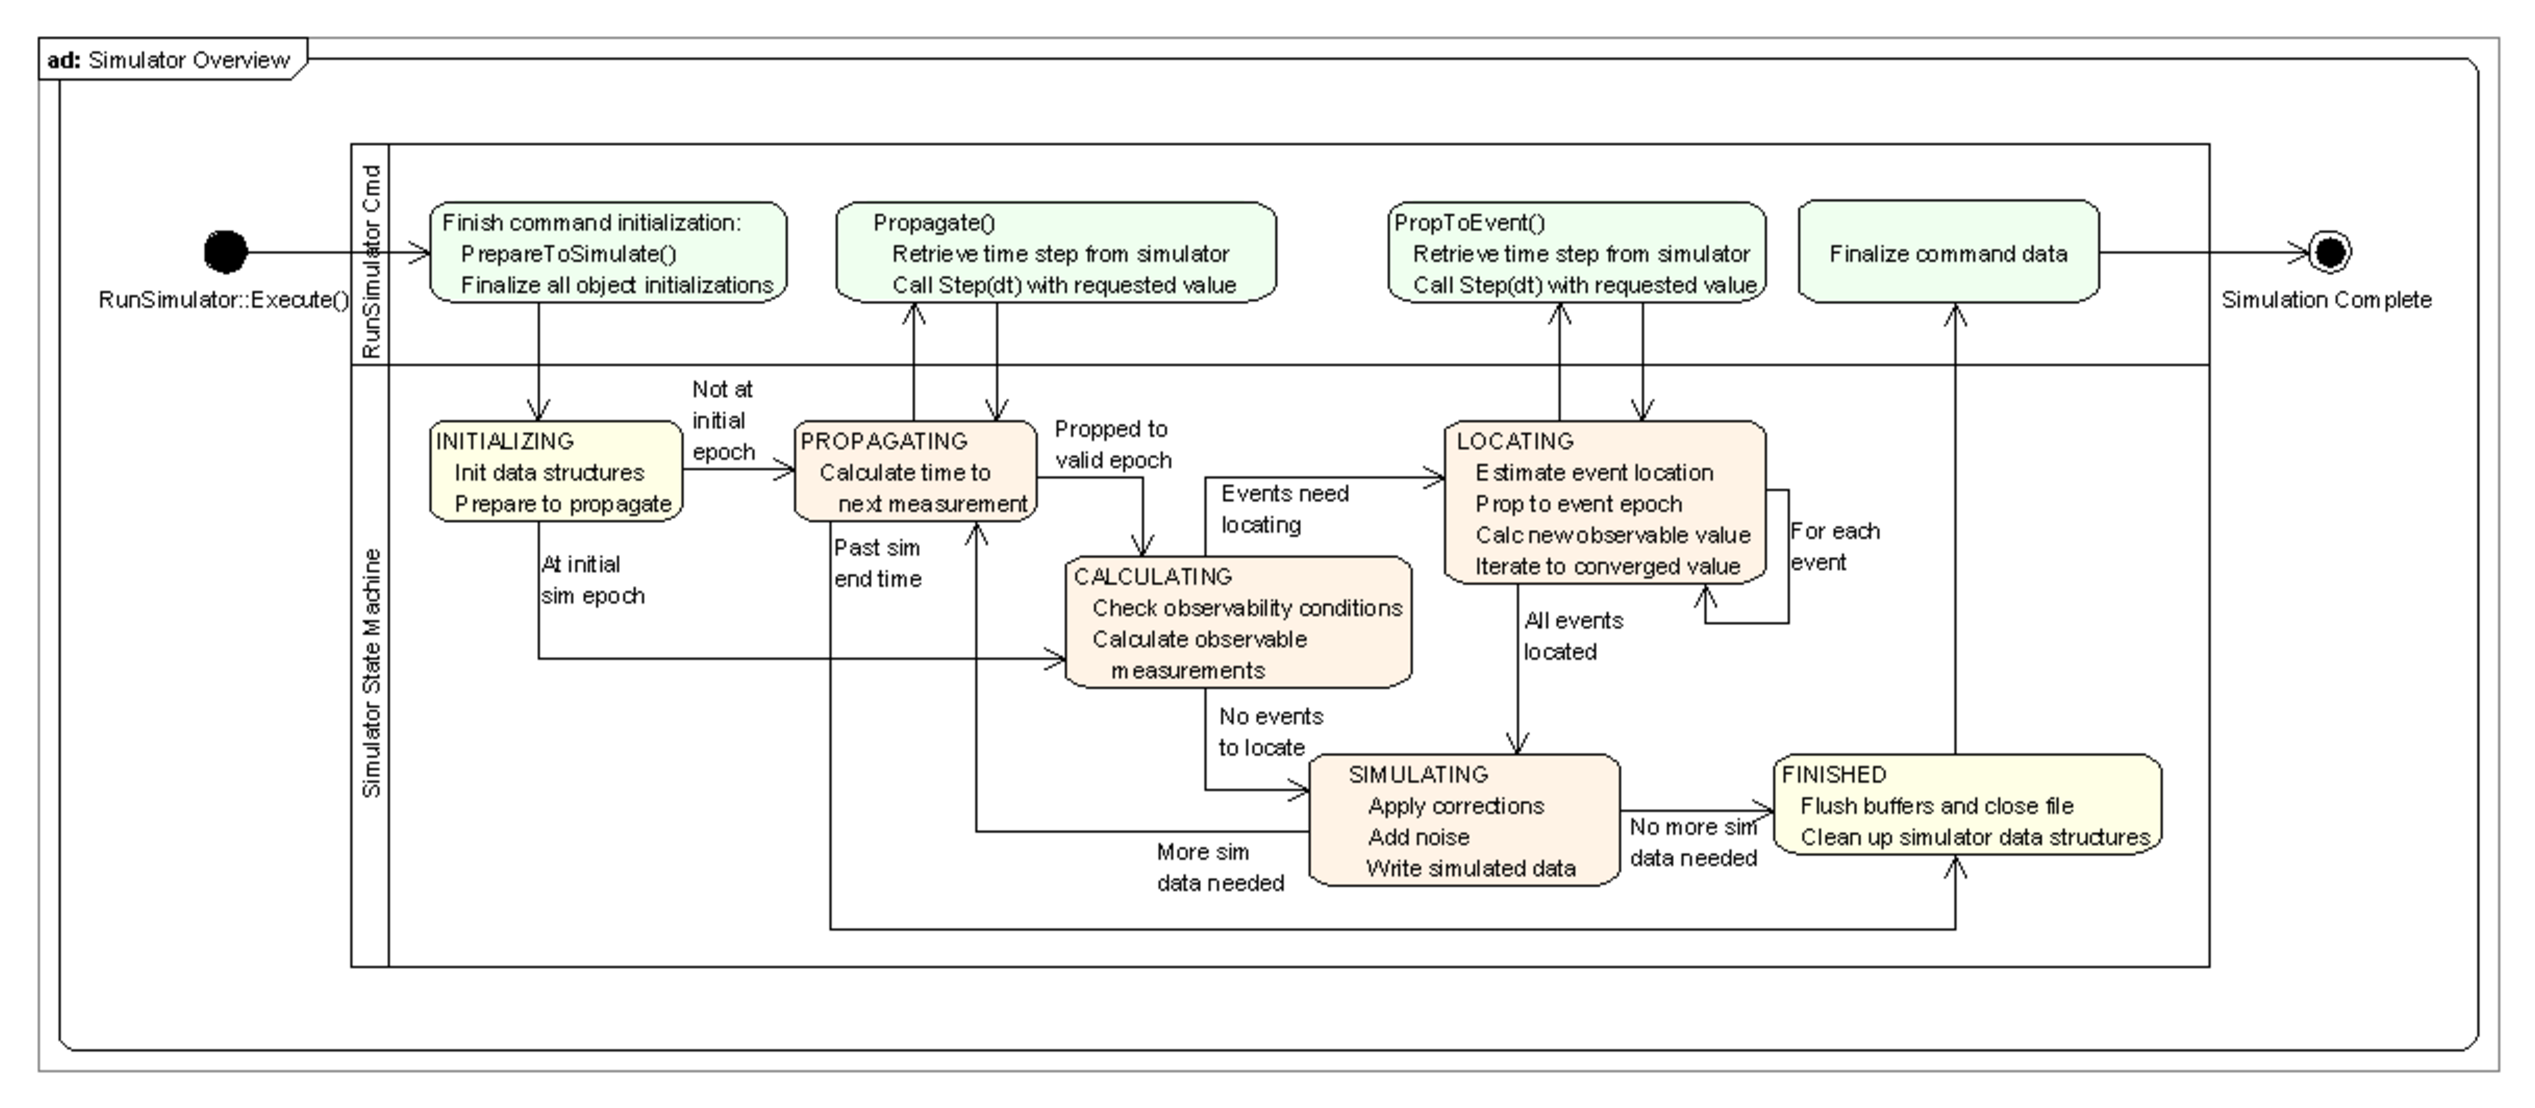
\includegraphics[scale=0.39]{Images/SimulatorOverview.eps}
\caption{\label{fig:SimulatorStateMachine}The Simulation State Machine}
\end{center}
\end{figure}

The list below describes each state of the machine, including the entry and exit conditions along with the internal actions required to move to the exit condition for the state:

\begin{description}
\item[INITIALIZING]\hspace{1pt}
\begin{itemize}
\item \textbf{Entry condition}
The INITIALIZING state is the state the Simulator takes upon completion of initialization in the Sandbox.  Upon completion of a simulation run, the Simulator returns to this state so that a subsequent call can reuse the same simulator.
\item \textbf{Actions} \textit{Method Name: CompleteInitialization()}
\begin{itemize}
\item Gather the data and fill the simulator's state.  Get current epoch from spacecraft participants, make sure all participants have the same epoch.  If not, throw an exception.
\end{itemize}
\item \textbf{Exit condition 1}:
\begin{itemize}
\item Change to PROPAGATING state if current epoch is not the simulation start epoch
\end{itemize}
\item \textbf{Exit condition 2}:
\begin{itemize}
\item Change to CALCULATING state if current epoch is the simulation start epoch
\end{itemize}
\end{itemize}
\item [PROPAGATING]\hspace{1pt}
\begin{itemize}
\item \textbf{Entry condition}:  A new observation needs to be simulated.
\item \textbf{Actions}		Method Name:  GetStepEpoch()
\begin{itemize}
\item Determine time step for propagation to the observation epoch
\item Provide time step to command for propagation on request
\item Determine if measurement for the observation has events that require propagation
\end{itemize}
\item \textbf{Exit condition 1}
\begin{itemize}
\item Propagation to the desired time has occurred
\item No unprocessed propagation events
\item Change state to CALCULATING
\end{itemize}
\item \textbf{Exit condition 2}
\begin{itemize}
\item Propagation to the desired time has occurred
\item Current epoch is past simulation end time
\item Change state to FINISHED
\end{itemize}
\end{itemize}
\item [LOCATING]\hspace{1pt}
\begin{itemize}
\item \textbf{Entry conditions}
\begin{itemize}
\item An event that requires propagation has been found
\item Resources are at a known epoch for the event, called the anchor epoch.
\end{itemize}
\item \textbf{Actions} \textit{Method Name:  ProcessEvent()}
\begin{itemize}
\item Manage the flag used to handle buffer state information
\item Calculate time step required for the event
\item Provide time step to command for propagation on request
\item Evaluate event to determine if propagation results are within tolerance
\item Iterate from time step calculation until event converges
\end{itemize}
\item \textbf{Exit condition 1}
\begin{itemize}
\item Event has converged
\item No additional events found
\item Reset state information to buffered data
\item Change state to SIMULATING
\end{itemize}
\item \textbf{Exit condition 2}
\begin{itemize}
\item Event has converged
\item Another event found
\item Change state to LOCATING and start a new iteration
\end{itemize}
\end{itemize}
\item [CALCULATING]\hspace{1pt}
\begin{itemize}
\item \textbf{Entry condition}:  Epoch is at a simulation epoch.
\item \textbf{Actions} Method Name:  CalculateParameters()
\begin{itemize}
\item Determine observability for measurements at the current epoch
\item Measurement manager gets and stores measurement values for the current epoch
\end{itemize}
\item \textbf{Exit condition 1}
\begin{itemize}
\item No measurements are observable
\item Change state to PROPAGATING
\end{itemize}
\item \textbf{Exit condition 2}
\begin{itemize}
\item At least one measurement primitive was calculated
\item No propagation is required for corrections
\item Change state to SIMULATING
\end{itemize}
\item \textbf{Exit condition 3}
\begin{itemize}
\item At least one measurement primitive was calculated
\item Corrections that require event finding were detected
\item Change state to LOCATING
\end{itemize}
\end{itemize}
\item [SIMULATING]\hspace{1pt}
\begin{itemize}
\item \textbf{Entry condition}:
All measurements and events at the current epoch have been pre-processed
\item \textbf{Actions} \textit{Method Name:  Simulate()}
\begin{itemize}
\item Apply corrections to all observable measurements
\item Tell measurement manager to write measurement data to the measurement data stream
\item Calculate the time step to the next measurement that needs to be simulated
\end{itemize}
\item \textbf{Exit condition 1}
\begin{itemize}
\item Measurement data was written to the data stream
\item Propagation time step remains within the simulation span
\item Change state to PROPAGATING
\end{itemize}
\item \textbf{Exit condition 2}
\begin{itemize}
\item Measurement data was written to the data stream
\item Propagation time step remains outside of the simulation span
\item Change state to FINISHED
\end{itemize}
\end{itemize}
\item [FINISHED]\hspace{1pt}
\begin{itemize}
\item \textbf{Entry condition}:  Simulation work finished
\item \textbf{Actions} \textit{Method Name:  RunComplete()}
\begin{itemize}
\item Clean up data structures
\item Flush and close the measurement data stream
\end{itemize}
\item \textbf{Exit condition}
\begin{itemize}
\item Change state to INITIALIZING so simulator is reentrant
\end{itemize}
\end{itemize}
\end{description}

\subsection{Simulator Members}

\paragraph{Simulator Attributes}

\begin{itemize}
\item \textbf{StringArray measurements}:  Names of the measurement models used in this simulator.
This array of names is passed to the MeasurementManager for processing.
\item \textbf{MeasurementManager measManager}:  The MeasurementManager for the simulator
\item \textbf{std::string propName}:  Name of the configured propagator used to evolve objects
during the simulation process.
\item \textbf{PropSetup *propagator}:  The propagator configured for the simulation.
\item \textbf{GmatEpoch simulationStart}:  The start epoch for the simulation.
\item \textbf{GmatEpoch simulationEpoch}:  The current epoch of the simulation.
\item \textbf{Real simulationDuration}:  The length of the simulation, in seconds.
\item \textbf{GmatState *simulationState}:  The state vector that is propagated.
\end{itemize}

\paragraph{Simulator Methods}

\begin{itemize}
\item \textbf{bool Initialize()}:  Validates reference objects and sets up all available interconnections in the simulator.
\item \textbf{Solver::SolverState AdvanceState()}:  Evaluates the status of the finite state machine and implements transitions between states.
\item \textbf{virtual void CompleteInitialization()}:  Performs the final initialization steps needed before executing the simulation.  This method is called when the finite state machine is in the INITIALIZING state, and completes the actions required to transition to the next state.
\item \textbf{virtual void GetStepEpoch()}:  Determines the time step to the next epoch for access by the RunSimulator command. This method is called when the finite state machine is in the PROPAGATING state.
\item \textbf{virtual void ProcessEvent()}:  Determines the next time step needed to manage event finding. This method is called when the finite state machine is in the LOCATING state.  It may be called repeatedly as the event finding algorithm seeks the location of one or more events.
\item \textbf{Real GetTimeStep()}:  Retrieves the most recently computed time step for use in propagation. This public method is called by the RunSimulator command to determine the desired propagation step size.
\item \textbf{Integer GetBufferingStatus()}:  Returns -1 if objects need to be restored from the buffered objects in the RunSimulator command, 0 if the buffers are not to be accessed, and +1 if the simulation objects need to be buffered.  This public method is called by the RunSimulator command to determine when buffer actions are needed.
\item \textbf{virtual void CalculateParameters()}:  Calculates measurement data in the measurement primitives. This method is called when the finite state machine is in the CALCULATING state.
\item \textbf{virtual void Simulate()}:  Calculates the fully corrected measurement values that are reported to the measurement data stream, and writes those data to the stream.  The measurement data stream can be either a file, a database, or a live data stream.  (The initial estimation builds of GMAT support the file option.)
\item \textbf{virtual void RunComplete()}:  Cleans up the data structures used during the
simulation, flushed the data buffers associated with the measurement data stream, and closes the
stream.
\end{itemize}
